\subsection{Feedback de los usuarios}
Para poder llevar a cabo un análisis de los resultados de la aplicación
de este proyecto, se ha realizado una prueba piloto con un grupo de integrantes
de Tecnalia. Estos han estado probando la herramienta durante un periodo de tiempo
de dos semanas, y han proporcionado feedback sobre su experiencia a través de
la siguiente encuesta de satisfacción.

\subsubsection{¿La documentación te resultó intuitiva?} 

Esta pregunta busca entender la facilidad de uso y claridad de la documentación proporcionada 
con la herramienta. La documentación es crucial para que los usuarios puedan 
aprender a utilizar la herramienta de manera efectiva y rápida, sin tener que 
buscar ayuda externa constantemente. La figura \ref{fig:sur_1} muestra que el 
60\% de los encuestados consideran 
la documentación muy intuitiva, mientras que el 40\% la encuentra 
mayormente intuitiva. No hubo respuestas indicando que la documentación es 
confusa. Estos resultados son positivos y sugieren que la documentación es 
en gran medida clara y fácil de usar se señala que hay áreas que podrían mejorarse. 

\begin{figure}[!h]
    \centering
    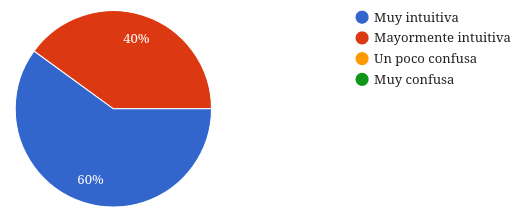
\includegraphics[width=0.8\textwidth]{sur_1.png}
    \caption{Resultado documentación de la herramienta.}
    \label{fig:sur_1}
\end{figure}

\subsubsection{¿Qué funcionalidad te ha parecido más útil?} 

Se busca identificar cuál de las funcionalidades ofrecidas por la 
herramienta ha sido la más valorada por los usuarios. Se refire a 
elementos concretos como los componentes, las plantillas y la gestión de
experimentos y datasets con ClearML. 
Los resultados indican que las funcionalidades más valoradas por los usuarios son 
plantillas y componentes, cada una con un 40\% de preferencia, mientras que 
ClearML es considerada útil por el 20\% de los encuestados. Esto sugiere que, aunque todas 
las funcionalidades tienen su utilidad, las plantillas y componentes son percibidas 
como las más valiosas.

\begin{figure}[!h]
    \centering
    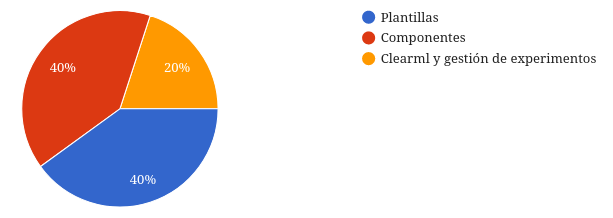
\includegraphics[width=0.8\textwidth]{sur_2.png}
    \caption{Resultado funcionalidades más valoradas.}
    \label{fig:sur_2}
\end{figure}


\subsubsection{¿Si tuvieras que contribuir a la documentación, que te gustaría aportar?}

Con esta pregunta se busca entender qué tipo de contribuciones estarían dispuestos
a hacer los usuarios de la herramienta. Se refiere a la creación de plantillas,
componentes, entradas de blog, o si por el contrario, no están interesados en contribuir.
Los resultados indican que el 60\% de los encuestados están dispuestos a contribuir 
a la documentación mediante la creación de plantillas o componentes. 
Mientras que otro 40\% no se ven contribuyendo a la documentación y nadie está interesado 
en contribuir con entradas de blog. Esto sugiere que, aunque hay interés en la creación 
de plantillas, un porcentaje significativo de usuarios no está dispuesto a contribuir 
en absoluto. Sería útil investigar las razones detrás de esta falta de interés en 
contribuir y buscar formas de incentivar la participación, especialmente en áreas como 
entradas de blog, que pueden ser muy útiles.

\begin{figure}[!h]
    \centering
    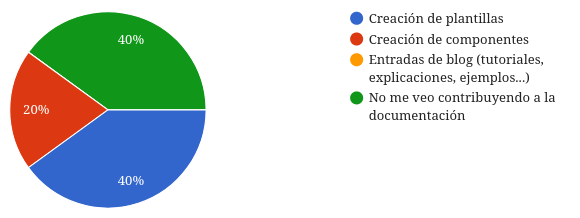
\includegraphics[width=0.8\textwidth]{sur_3.png}
    \caption{Resultado contribución a la documentación.}
    \label{fig:sur_3}
\end{figure}


\subsubsection{¿Cuánto tiempo al mes podrías dedicar a contribuir?}

Con la siguiente cushion se busca medir el compromiso potencial de los usuarios con la 
herramienta. Se refiere al tiempo que los usuarios estarían dispuestos a invertir 
en contribuir con feedback, desarrollo, documentación, o cualquier otra 
forma de colaboración. 
Los resultados indican que el 40\% de los encuestados están dispuestos a dedicar menos 
de 30 minutos al mes para contribuir, y otro 40\% está dispuesto a dedicar entre 30 
minutos y 1 hora. Un 20\% de los encuestados podría dedicar entre 1 y 3 horas, 
mientras que ninguno está dispuesto a dedicar más de 3 horas. Esto sugiere que la 
mayoría de los usuarios tienen un tiempo limitado para contribuir y es importante 
tener en cuenta este factor al diseñar oportunidades de contribución.

\begin{figure}[!h]
    \centering
    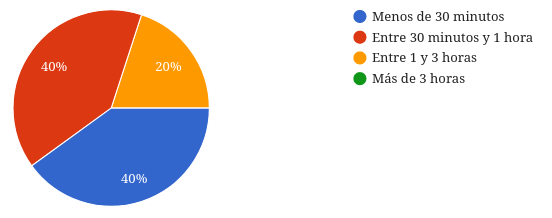
\includegraphics[width=0.8\textwidth]{sur_4.png}
    \caption{Resultado tiempo dedicado a contribuir.}
    \label{fig:sur_4}
\end{figure}


\subsubsection{¿Has utilizado anteriormente alguna plataforma MLOPs?}

Se investiga el nivel de experiencia previa de los usuarios con plataformas 
similares de MLOps. Saber si los usuarios tienen experiencia previa ayuda 
a contextualizar sus respuestas y expectativas. Los resultados indican que el 60\% de 
los encuestados creen que la herramienta agiliza mucho su trabajo, mientras que el 40\% no 
la ha utilizado pero le gustaría incorporarla. Estos resultados son muy positivos y sugieren una 
percepción general favorable de la herramienta. Para aquellos interesados 
en incorporarla, sería beneficioso proporcionar recursos y apoyo para facilitar 
su adopción, asegurando así una integración exitosa y mejorando aún más la 
eficiencia del trabajo.

\begin{figure}[!h]
    \centering
    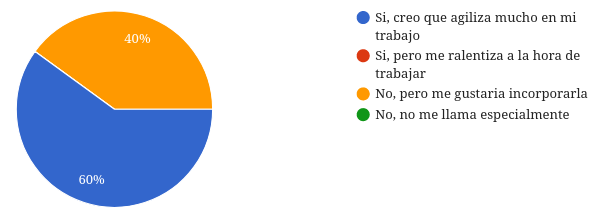
\includegraphics[width=0.8\textwidth]{sur_5.png}
    \caption{Previsualización del componente show\_time\_series\_compare}
    \label{fig:sur_5}
\end{figure}

\subsubsection{¿Qué te parece la gestión de datasets de ClearML?} 

Esta pregunta está 
enfocada en recoger opiniones sobre una funcionalidad específica de la 
herramienta, en este caso, la gestión de datasets que ofrece ClearML. 
Se busca entender cómo los usuarios perciben esta funcionalidad en términos 
de usabilidad.
Los resultados indican que el 60\% de los encuestados encuentran la herramienta 
útil pero complicada, mientras que el 40\% tablen la encuentra útil pero la considera 
sencilla. Estos resultados sugieren que, aunque la herramienta tiene un valor 
percibido positivo, su complejidad puede ser una barrera para su uso efectivo. 

\begin{figure}[!h]
    \centering
    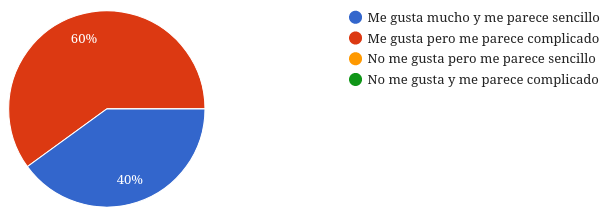
\includegraphics[width=0.8\textwidth]{sur_6.png}
    \caption{Previsualización del componente show\_time\_series\_compare}
    \label{fig:sur_6}
\end{figure}


\subsubsection{¿Qué te parece la gestión de experimentos de ClearML?}
Similar a la pregunta anterior, esta está diseñada para obtener opiniones 
sobre otra funcionalidad específica: la gestión de experimentos. Se busca 
evaluar cómo los usuarios perciben la capacidad de la herramienta para 
gestionar y monitorizar experimentos de machine learning.
Los resultados indican que el 80\% de los encuestados les gusta mucho la 
herramienta y la encuentran sencilla de usar, mientras que el 20\% la encuentra 
útil pero complicada. No hubo respuestas indicando que no les gusta la herramienta, 
ya sea que la encuentren sencilla o complicada. Estos resultados son muy positivos y 
sugieren que la gran mayoría de los usuarios están satisfechos con la herramienta y 
la consideran fácil de usar. Sin embargo, todavía hay un pequeño porcentaje que 
encuentra la herramienta complicada, por lo que sería beneficioso identificar 
las áreas específicas que pueden ser simplificadas para mejorar la experiencia de 
todos los usuarios.

\begin{figure}[!h]
    \centering
    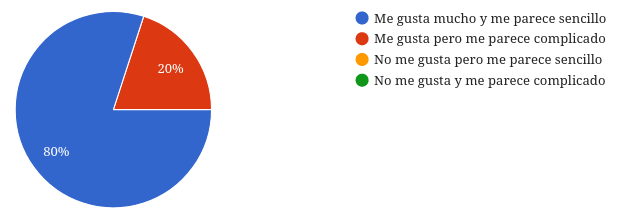
\includegraphics[width=0.8\textwidth]{sur_7.png}
    \caption{Previsualización del componente show\_time\_series\_compare}
    \label{fig:sur_7}
\end{figure}


\subsection{Valoración general}
Los resultados de la encuesta reflejan una percepción general muy positiva de la 
herramienta. La mayoría de los usuarios encuentran la documentación intuitiva y 
útil, especialmente destacando la facilidad de uso de las plantillas y componentes. 
Además, muchos consideran que esta agiliza significativamente su trabajo, lo cual 
es un indicador claro de su valor y efectividad en mejorar la eficiencia laboral. 
La disposición de algunos usuarios a contribuir a la documentación, aunque sea en 
pequeñas cantidades de tiempo, también es un buen signo de compromiso y apoyo.
A pesar de la percepción general positiva, existen áreas que necesitan mejoras. 
Un número considerable de usuarios encuentra complicaciones en ciertas areas, 
lo que sugiere que la complejidad puede ser una barrera para su uso efectivo. 
Además, hay una notable falta de interés en contribuir mediante la creación de 
entradas de blog, lo que podría indicar que esta forma de contribución no está 
suficientemente incentivada o explicada. También, aunque muchos encuentran la 
herramienta útil, algunos usuarios no se ven contribuyendo a la documentación en 
absoluto, lo que podría reflejar una falta de claridad sobre cómo pueden ayudar 
o un desinterés en el proceso.\medskip

En resumen, la encuesta muestra que la herramienta es bien recibida y 
valorada por su capacidad para facilitar el trabajo, aunque la complejidad 
percibida por algunos usuarios señala áreas de mejora. Enfocarse en simplificar 
la herramienta y fomentar formas diversas y accesibles de contribución podría 
aumentar aún más la satisfacción y el compromiso de los usuarios. Es crucial 
continuar recopilando feedback específico para orientar mejor las mejoras y 
mantener el alto nivel de satisfacción alcanzado hasta ahora.